\documentclass[a4paper,14pt]{extarticle}
\usepackage{../../tex-shared/preamble}

\renewcommand{\mylabnumber}{3}
\renewcommand{\mylabtitle}{Расчет числовых характеристик и 
                           энтропии непрерывной случайной величины}
\renewcommand{\mysubject}{Теория информационных процессов и систем}
\renewcommand{\mylecturer}{Заикина Е.Н.}

\begin{document}
\begin{titlepage}
    
    \thispagestyle{empty}
    
    \begin{center}
        
        Министерство науки и Высшего образования Российской Федерации \\
        Севастопольский государственный университет \\
        Кафедра ИС
        
        \vfill

        Отчет \\
        по лабораторной работе №\mylabnumber \\
        \enquote{\mylabtitle} \\
        по дисциплине \\
        \enquote{\MakeTextUppercase{\mysubject}}

    \end{center}

    \vspace{1cm}

    \noindent\hspace{7.5cm} Выполнил студент группы ИС/б-17-2-о \\
    \null\hspace{7.5cm} Горбенко К. Н. \\
    \null\hspace{7.5cm} Проверил \\
    \null\hspace{7.5cm} \mylecturer

    \vfill

    \begin{center}
        Севастополь \\
        \the\year{}
    \end{center}

\end{titlepage}
\section{Цель работы}
\begin{itemize}
    \item Изучение способов описания непрерывных случайных величин.
    \item Приобретение практических навыков расчета числовых характеристик
          и энтропии непрерывной случайной величины по ее плотности 
          распределения вероятности.
\end{itemize}

\section{Задание на работу}
Ход данной лабораторной работы аналогичен ходу лабораторной работы
№1; поскольку рассмотрению подлежит непрерывная случайная величина,
а не дискретная, то ряд распределения заменяется плотностью распределения,
а энтропия – дифференциальной энтропией.

\section{Ход работы}
Выберем закон распределения Рэлея:
\begin{equation*}
    p(x) = \frac{x}{\sigma^2} \cdot \exp{(-\frac{x^2}{2\sigma^2})}.
\end{equation*}

Опишем ограничения, накладываемые на параметры распределения и функцию,
определяющую плотность распределения вероятностей, проверим выполнение
условия нормировки:
\begin{figure}[H]
    \centering
    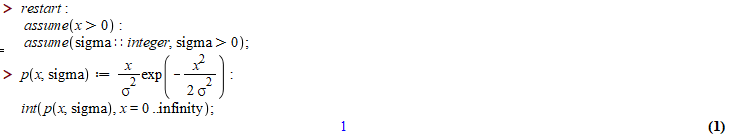
\includegraphics[width=\linewidth]{function}
    \caption{Функция плотности вероятностей}
    \label{fig:function}
\end{figure}

Опишем функции вычисления начального момента порядка s и математического ожидания:
\begin{figure}[H]
    \centering
    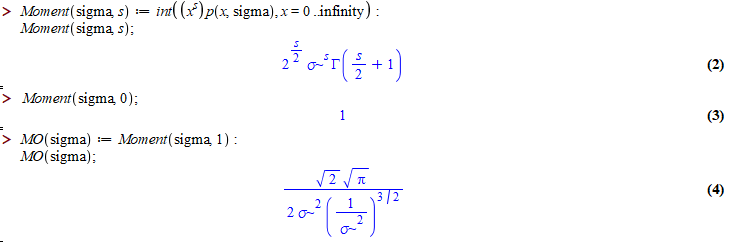
\includegraphics[width=\linewidth]{alpha}
    \caption{Начальный момент и математическое ожидание}
    \label{fig:alpha}
\end{figure}

График зависимости математического ожидания от $\sigma$ изображен на рисунке \ref{fig:mo}
\begin{figure}[H]
    \centering
    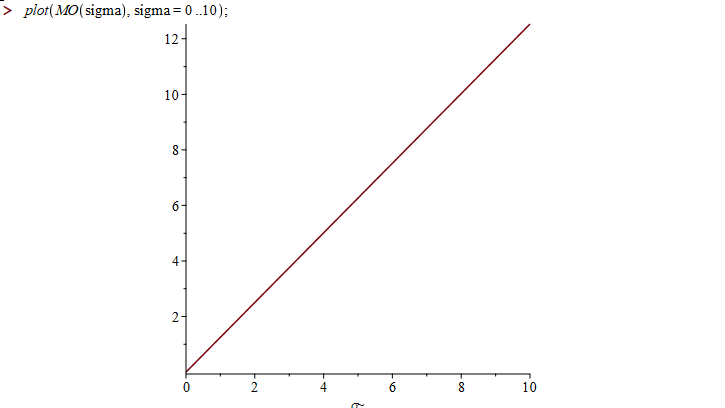
\includegraphics[width=\linewidth]{mo}
    \caption{График зависимости математического ожидания от $\sigma$}
    \label{fig:mo}
\end{figure}

Опишем функцию вычисления центрального момента порядка s:
\begin{figure}[H]
    \centering
    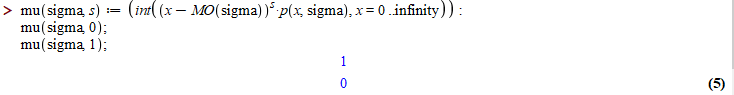
\includegraphics[width=\linewidth]{mu}
    \caption{Центральный момент порядка s}
    \label{fig:mu}
\end{figure}

Опишем функцию вычисления дисперсии. Построим график ее зависимости от $\sigma$:
\begin{figure}[H]
    \centering
    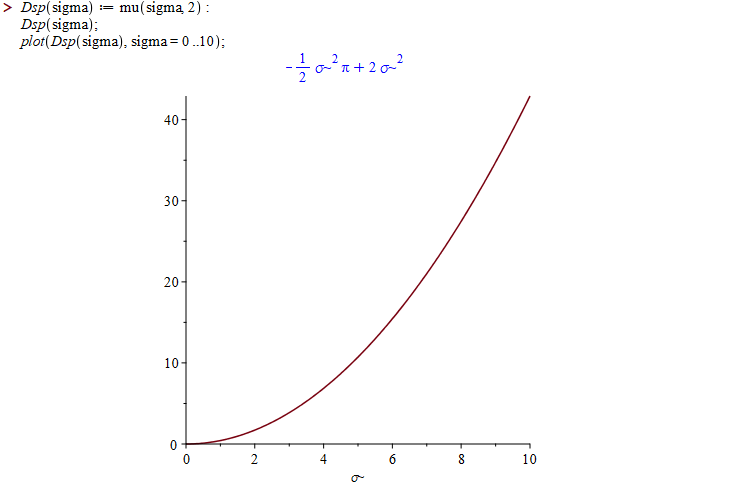
\includegraphics[width=\linewidth]{disp}
    \caption{График зависимости дисперсии от $\sigma$}
    \label{fig:disp}
\end{figure}

Опишем функцию вычисления среднеквадратического отклонения. Построим график
его зависимости от $\sigma$:
\begin{figure}[H]
    \centering
    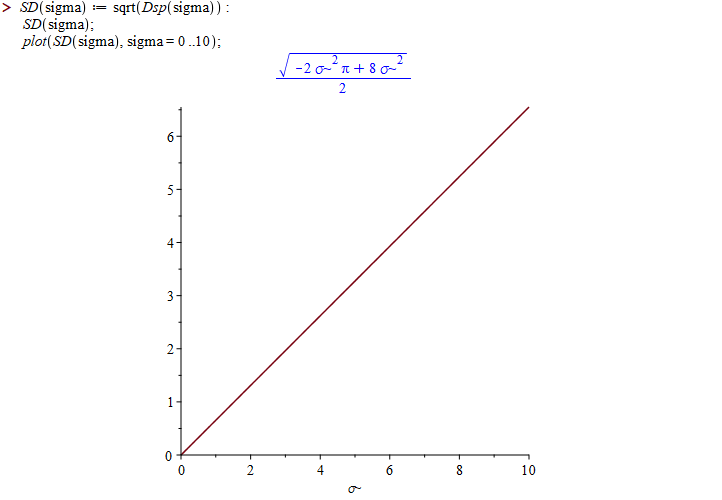
\includegraphics[width=\linewidth]{sko}
    \caption{График зависимости среднеквадратического отклонения от $\sigma$}
    \label{fig:sko}
\end{figure}

СКО закона распределения Рэлея линейно зависит от $\sigma$.

Опишем функцию вычисления коэффициента ассиметрии. Построим график его
его зависимости от $\sigma$:
\begin{figure}[H]
    \centering
    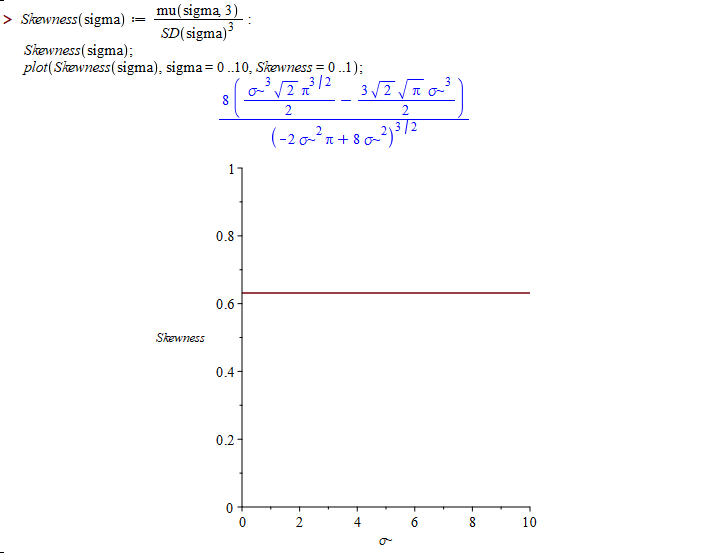
\includegraphics[width=\linewidth]{skewness}
    \caption{График зависимости коэффициента ассиметрии от $\sigma$}
    \label{fig:skewness}
\end{figure}

Опишем функцию вычисления коэффициента эксцесса. Построим график его
его зависимости от $\sigma$:
\begin{figure}[H]
    \centering
    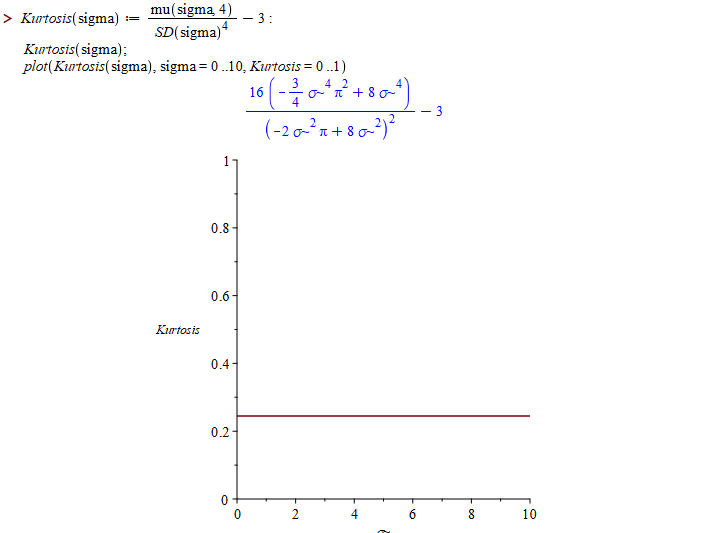
\includegraphics[width=\linewidth]{kurtosis}
    \caption{График зависимости коэффициента эксцесса от $\sigma$}
    \label{fig:kurtosis}
\end{figure}

Коэффициенты ассиметрии и эксцесса не зависят от $sigma$.

Построим графики плотности вероятностей для различных $\sigma$.
\begin{figure}[H]
    \centering
    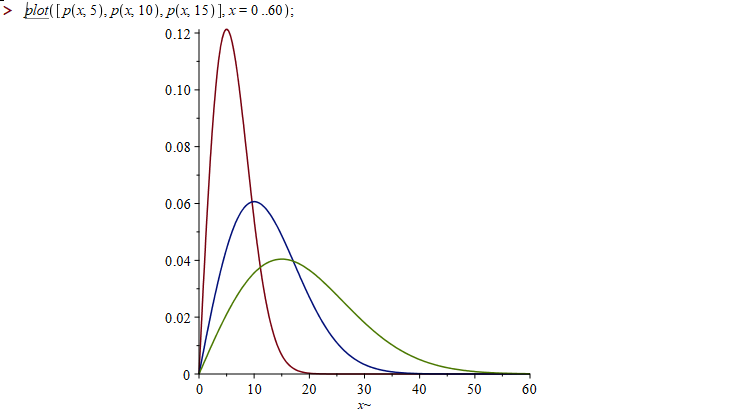
\includegraphics[width=\linewidth]{pdf}
    \caption{Графики плотности вероятностей при $\sigma$ = 5, $\sigma$ = 10, $\sigma$ = 15}
    \label{fig:pdf}
\end{figure}

Опишем функцию вычисления интегральной функци распределения.
Построим ее графики для различных $\sigma$:
\begin{figure}[H]
    \centering
    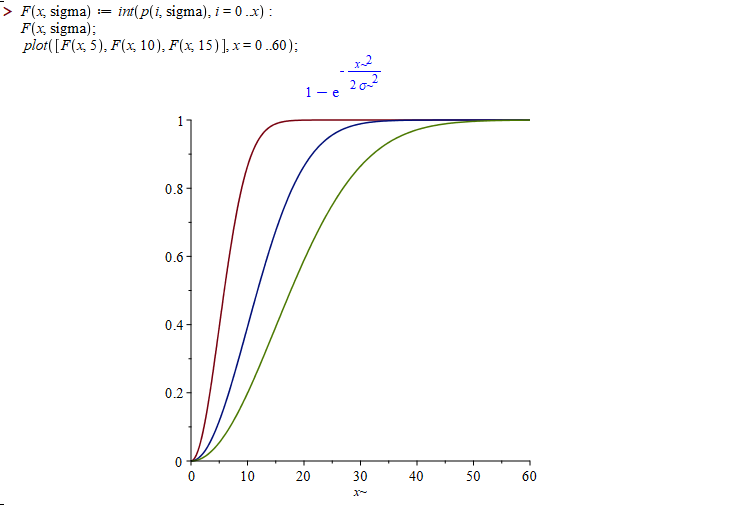
\includegraphics[width=\linewidth]{integral}
    \caption{Графики интегральной функции при $\sigma$ = 5, $\sigma$ = 10, $\sigma$ = 15}
    \label{fig:integral}
\end{figure}

Опишем функцию вычисления дифференциальной энтропии. Построим график 
ее зависимости от $\sigma$
\begin{figure}[H]
    \centering
    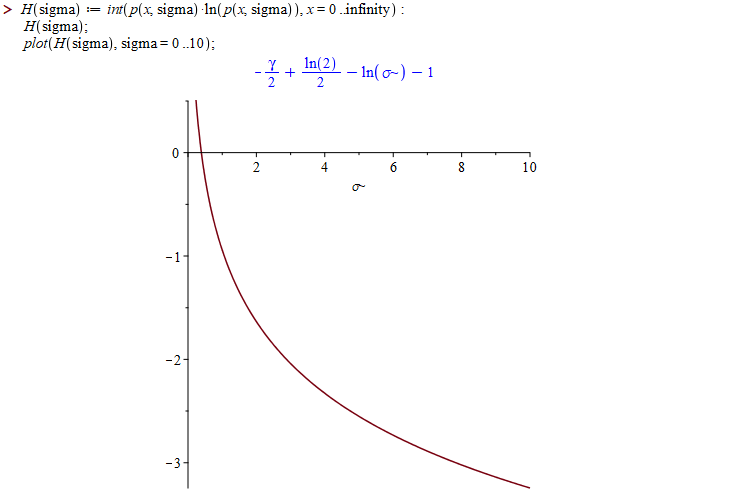
\includegraphics[width=\linewidth]{entropy}
    \caption{График зависимости дифференциальной энтропии от $\sigma$}
    \label{fig:entropy}
\end{figure}

Дифференциальная энтропия принимает отрицательные значения в промежутке [0.4; $\infty$]

\section*{Вывод}
В ходе лабораторной работы был исследован закон распределения Рэлея.
Он имеет параметр $\sigma$, характеризующий масштаб распределения.
СКО случайной величины, распределенной по данному закону, линейно зависит от
параметра $\sigma$, а дисперсия квадратично. Коэффициенты ассиметрии и эксцесса
не зависят от $\sigma$. 
\end{document}